% -----------------------------------------------------------------------------
%   Arquivo: ./02-elementos-textuais/trabalhosRelacionados.tex
% -----------------------------------------------------------------------------



\chapter{O pacote MLAT }
\label{chap:TheSoftware}
A tarefa de criação de um novo modelo de aprendizado de máquina passa por algumas etapas bem definidas, como, implementação, \textit{benchmarking} e análise de resultados, conforme mostra o diagrama da figura \ref{fig:BuildingMLModel}.

\begin{figure}[!htb]
	\centering
	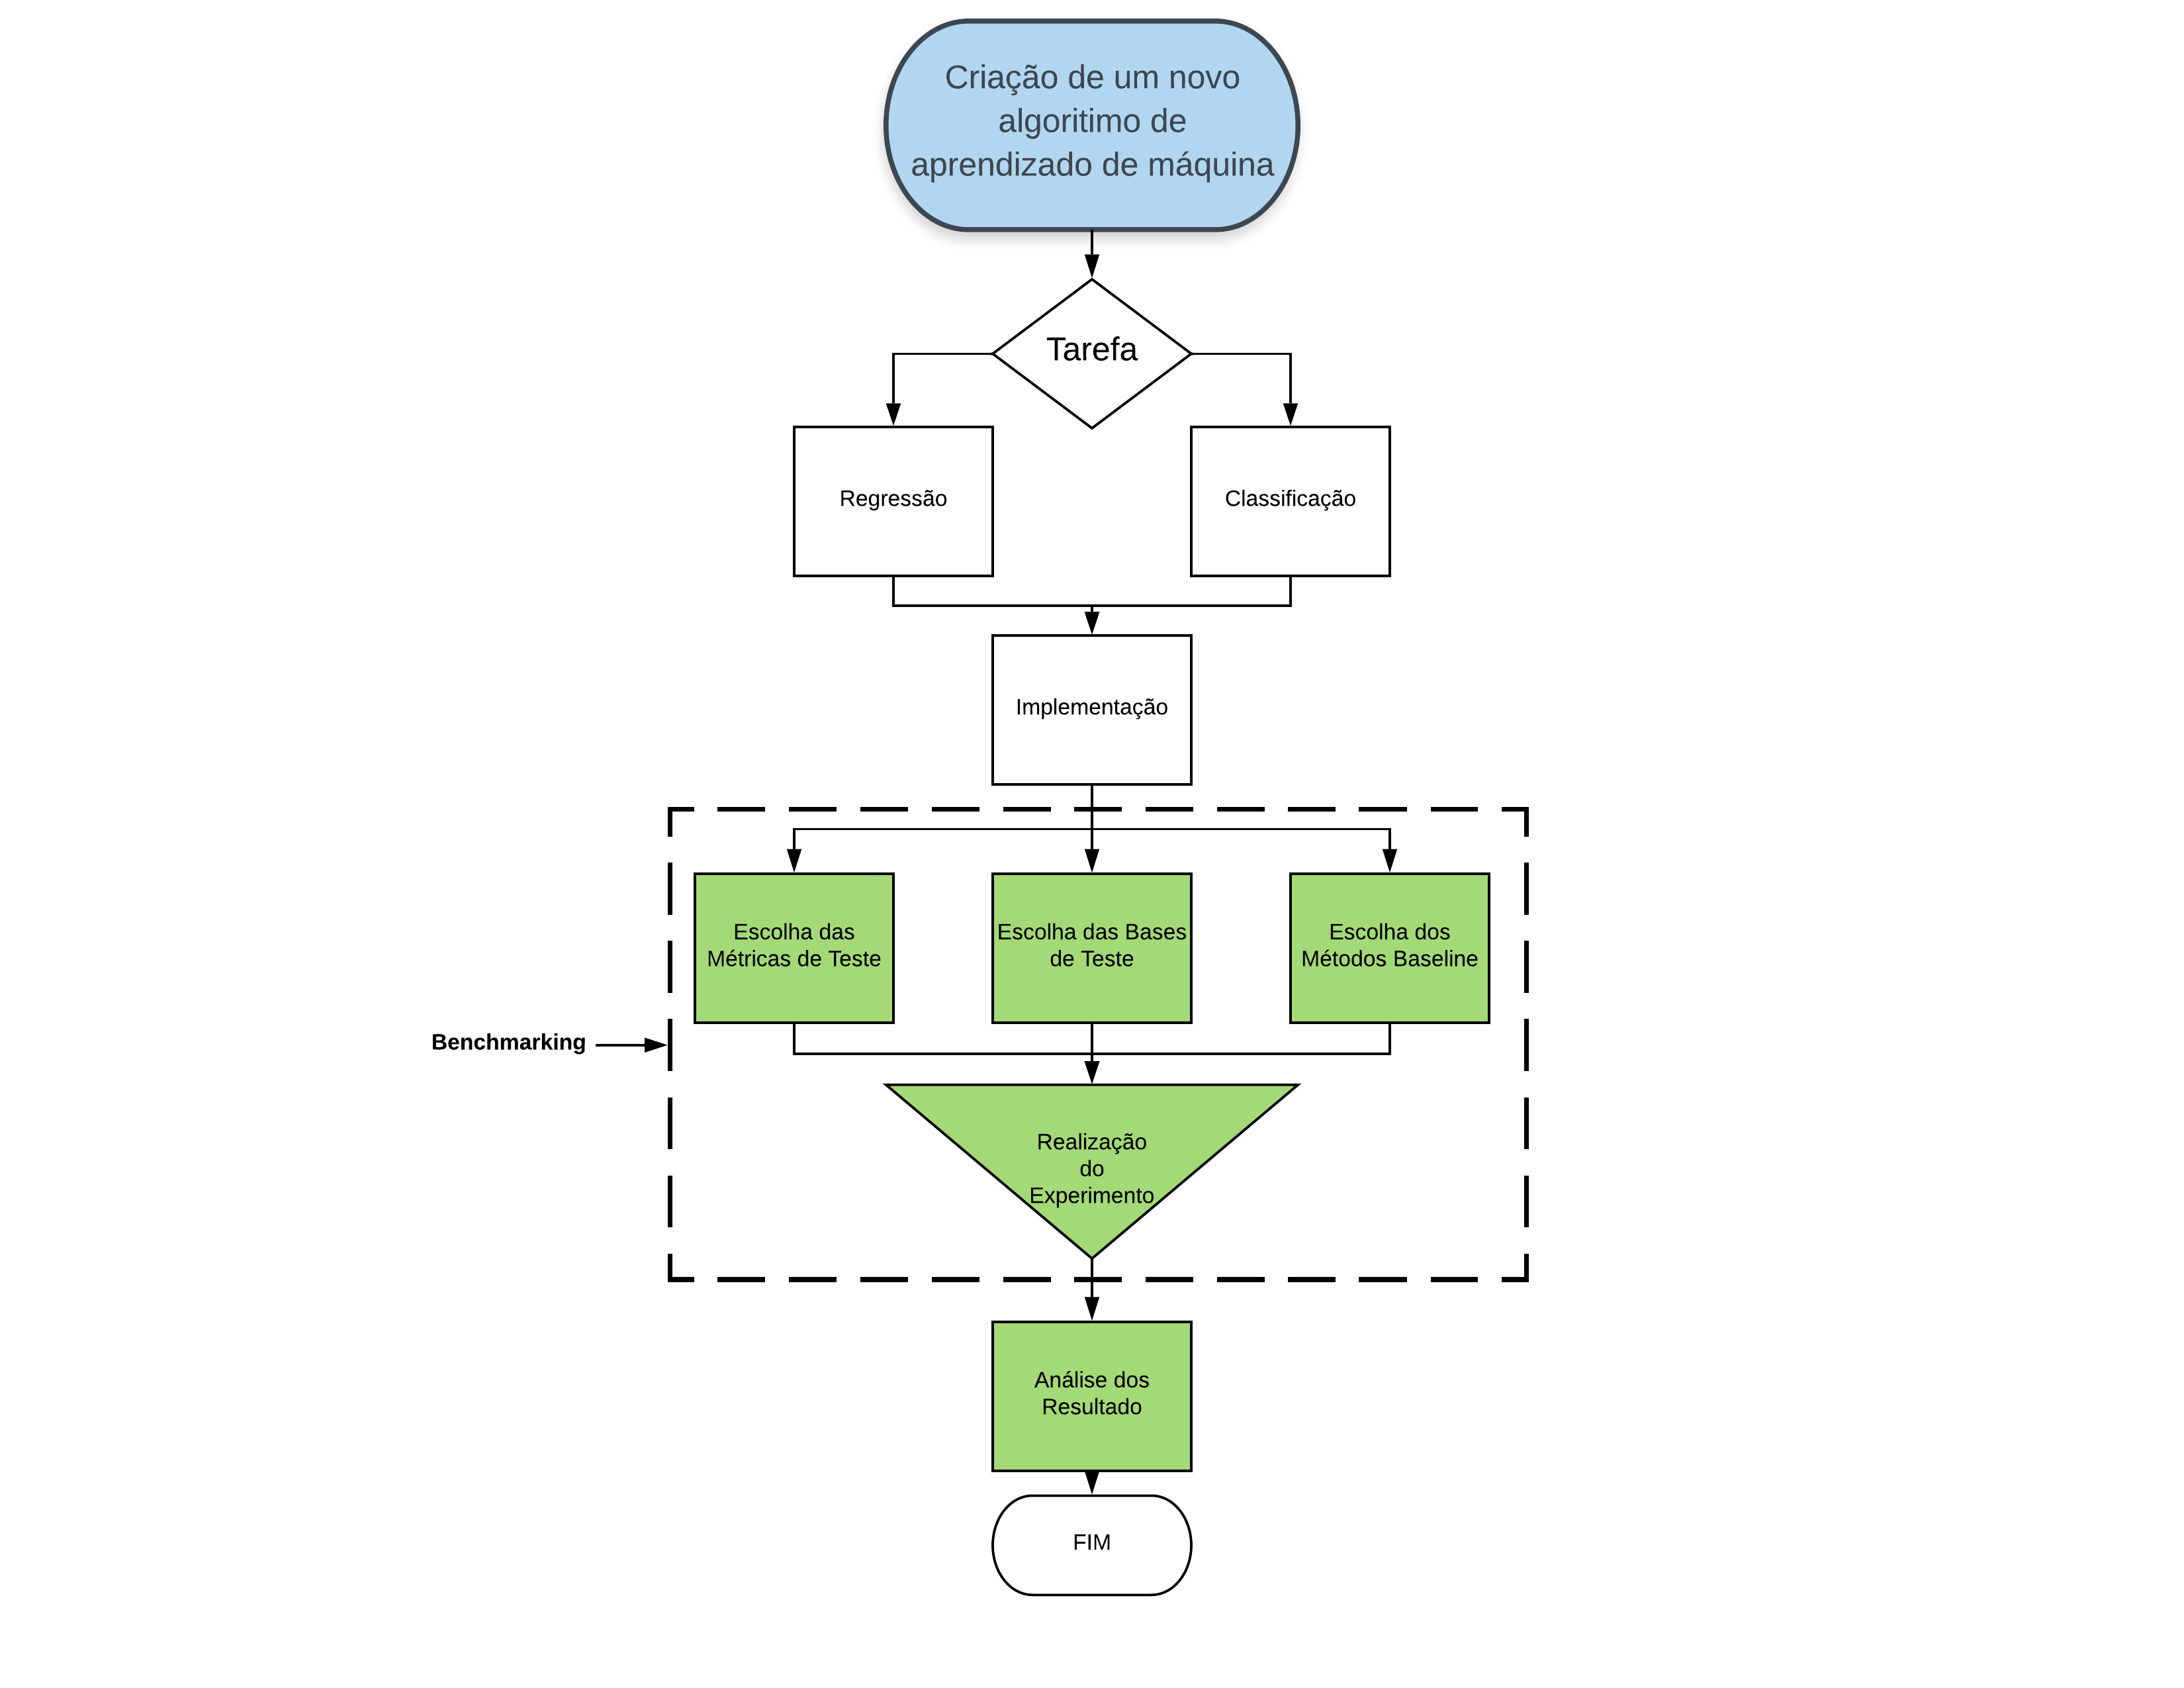
\includegraphics[width=\textwidth]{./04-figuras/BuildingNewMethod.png}
	\caption{Etapas da construção de um novo modelo de aprendizado.} 
	\label{fig:BuildingMLModel}
\end{figure}

O pacote \textit{Machine Learning Atutomated Testing} (MLAT) têm como objetivo automatizar e simplificar algumas dessas etapas, representadas de verde no diagrama da figura \ref{fig:BuildingMLModel}. 

Nesse capítulo será descrito cada uma dessas etapas e como, o pacote MLAT, vai auxiliar seus usuários em cada uma delas. Por fim, será apresentado a forma de utilização do pacote e uma implementação exemplo.

\section{Métodos Baseline}
\label{sec:Metodos}
Os métodos baseline foram divididos em três grupos : regressão, classificação binário ou \textit{multylabel}. Foi importante dividir os métodos nesses três grupos porque o mesmo foi feito para as bases de dados e métricas de teste. Essa decisão de projeto possibilitou uma simplicidade na interface do usuário, em que ele apenas informa o programa a tarefa e é possível obter todos os métodos, bases e métricas que serão possíveis de serem utilizadas.

No MLAT foram implementados, inicialmente, os métodos descritos no capítulo \ref{chap:MachineLearning} para as três tarefas citadas acima. O pacote fornece uma interface que o usuário pode apenas informar a tarefa e o programa retorna uma lista com os métodos e suas parametrizações padrão, ou ainda, o usuário pode criar uma lista com os métodos e suas próprias parametrizações. 

\section{Métricas de Testes}
\label{sec:Metricas}
Todo algorítimo de aprendizado de máquina, implicitamente ou explicitamente, tem como objetivo minimizar algum tipo de erro. Todavia, o erro minimizado, pode ser diferente entre os modelos, ou ainda, não representar o verdadeiro objetivo do aprendizado. Dessa maneira, durante a comparação entre os modelos de aprendizado, é importante definir a priori métricas representatívas do verdadeiro objetivo do aprendizado, para ser possível comparar os modelos da maneira justa.

Para fazer isso, o pacote MLAT, permite ao usuário escolher entre mais de 20 possíveis métricas de avaliação divididas em três tarefas. Para utilizar qualquer uma das métricas, o usuário, precisa informar ao pacote os nomes das métricas desejadas ou escolher entre as tarefas de regressão, classificação binária ou \textit{multylabel}.

\section{Bases de Teste}
\label{sec:Bases}
Algumas bases de dados, como MNIST \cite{lecun} ou \textit{Spam or Ham} \cite{zezim}, se tornaram problemas clássicos para se comparar o desempenho de novos modelos de aprendizado de máquina. Com o objetivo de poupar o usuário da busca e preparo das bases de dados clássicas, foi implementado no pacote uma forma de carregamento em que ele apenas informa os nomes das bases ou a tarefa de aprendizado. Após a escolha das bases o pacote aplica os modelos em cada uma das bases de maneira autônoma, informando o usuário apenas as métricas de testes.

É importante salientar, que nessa versão do pacote, é possível serem utilizadas apenas as bases de disponibilizadas. Essa foi uma decisão de projeto que garantiu um funcionamento mais otimizado do pacote e que possibilitou uma interface mais simples para o usuário. 

Até o momento foram disponibilizadas 20 bases, e na próxima versão do MLAT, haverá uma interface que possibilitará a adição de qualquer base por meio de uma função que à colocará no padrão do pacote.

\section{Realização do Experimento}
A realização do experimento culmina na combinação das três etapas anteriores, descritas nas seções \ref{sec:Metodos}, \ref{sec:Metricas} e \ref{sec:Bases}. Nesse momento o usuário pode informar ao programa alguns parâmetros do teste, como o percentual do \textit{split} entre treino e teste, e o número de vezes que cada teste será realizado para os pares de algoritmo e parametrização. Ao fim do processo é entregue ao usuário uma tabela que contêm todos as métricas dos resultados de cada iteração de teste.

\section{Análise dos  Resultados}
A etapa de análise dos resultados é o momento em que o projetista deve escolher uma métrica objetivo para que ele possa comparar os diferentes métodos treinados. A saida desse momento deve ser capaz de auxiliar o projista no julgamento de qual método tever melhor desempenho no experimento. Para cumprir esse objetivo, o pacote permite ao usuário escolher e performar um dos testes estatísticos descritos no capítulo \ref{chap:testStatistics}. 



\section{Uso do MLAT}

\begin{figure}[!htb]
	\centering
	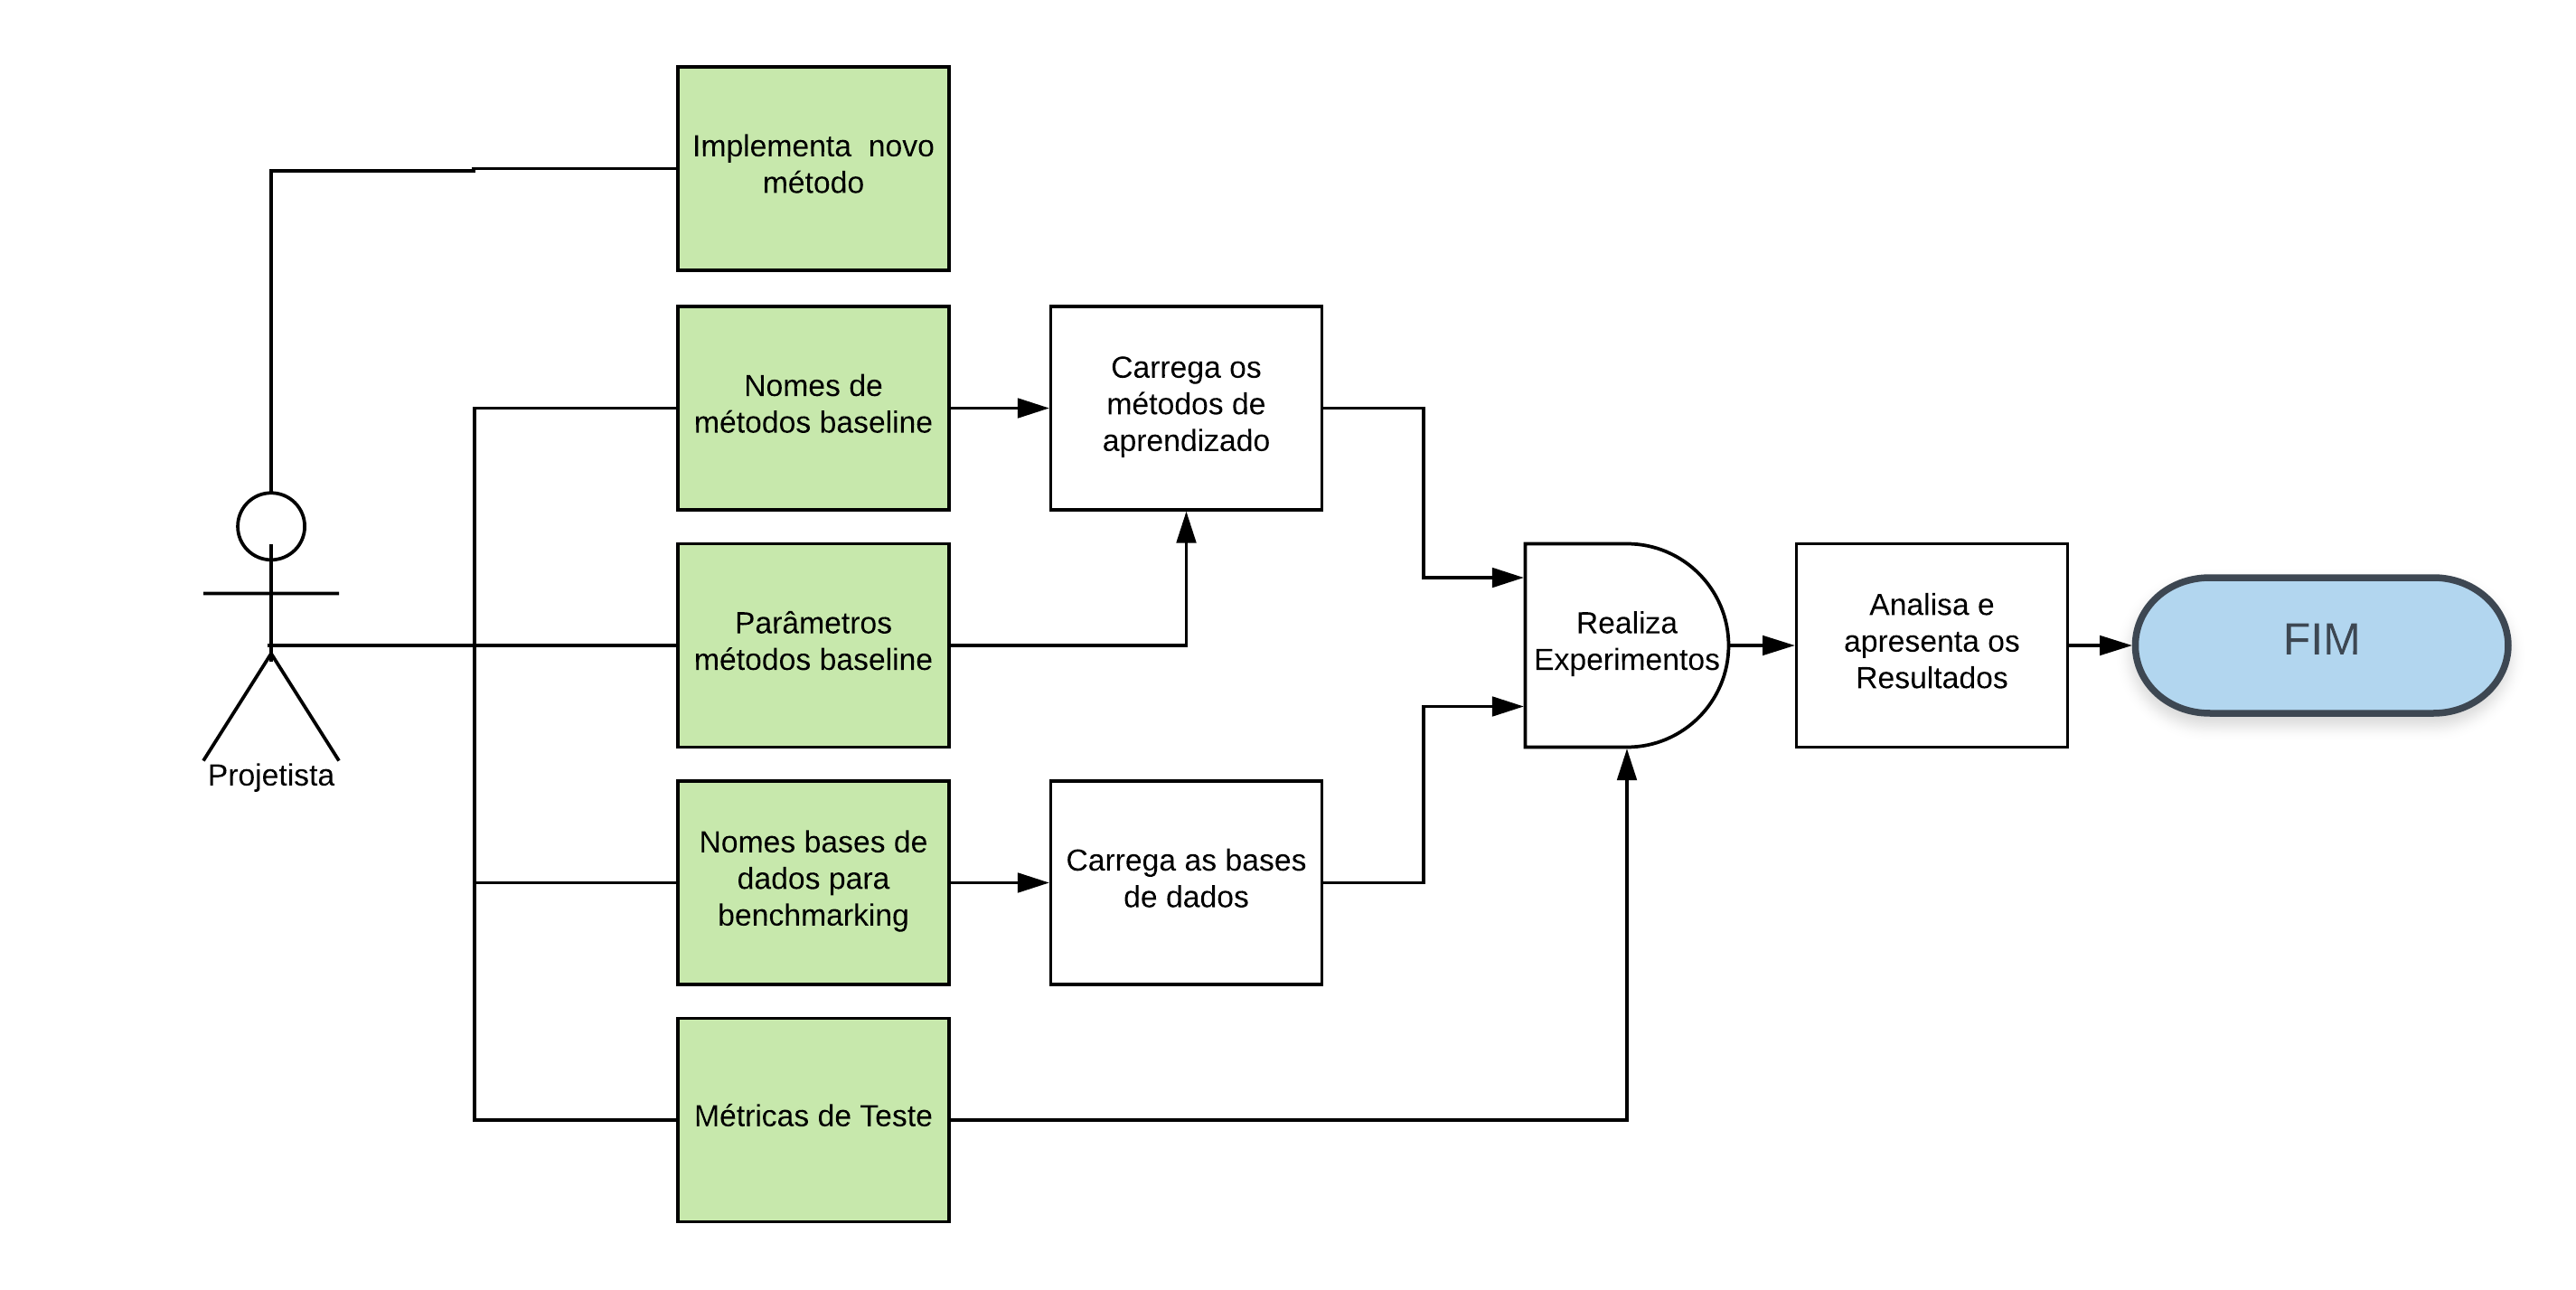
\includegraphics[width=\textwidth]{./04-figuras/UseCase.png}
	\caption{Utilização do Pacote MLAT.} 
	\label{fig:BuildingMLModel}
\end{figure}


\begin{lstlisting}[language=R]

### Carrega e instala pacotes
install.packages('devtools')
require('devtools')
devtools::install_github('PauloCirino/MLAT')
require('MLAT')

### O novo algoritmo
MyNewAlgoFunc <- function(X_train, Y_train, X_test, k) {
Y_hat <- numeric()
for( i in 1:nrow(X_test)){
x_iter <- X_test[i, ]
distVet <- apply(X_train, 1, function(x){
sum( abs(x_iter - x ) )
})
Y_iter_vet <- Y_train[ order(distVet) ] [1:k]
Y_iter_aux <- numeric()
for(j in 1:k){
Y_iter_aux <- append(Y_iter_aux,
rep(Y_iter_vet[j],
k - j + 1) )
}
unique_y <- unique(Y_iter_aux)
aux_Table <- tabulate(match(Y_iter_aux,  unique_y))
Y_hat[i] <- unique_y[which.max(aux_Table)]
}
Y_hat
}

### Parametriza teste
task <- 'MultClass'
cmpTestsFuncsList <- MLAT::GetAllMultClassAlgo()
dataSetNames <- MLAT::GetDataSetsNames(task = task)
testMetrics <- MLAT::GetMetrics(task = task)

### Coloca minha funcao no padrao do pacote
newAlgoInStandarts <- MLAT::CreateAlgo(  
algoName = 'KNN Mahalanobis Ponderado', 
algoFun = MyNewAlgoFunc, 
task = task, 
paramList = list(k = 2:10) )
cmpTestsFuncsList[[length(cmpTestsFuncsList) + 1]] <- newAlgoInStandarts

### Realiza experimento
myResult <- RunTests( cmpTestsFuncsList = cmpTestsFuncsList,
task = task,
dataSetNames = dataSetNames,
metrics = testMetrics,
nTestsPerParam = 10,
splitPerc = 0.7, 
verbose = TRUE)

\end{lstlisting}

